
\marginpar{\href{https://youtu.be/j9WZyLZCBzs}{Video}} Read sections: 1.1, 1.2\\
\marginpar{\href{https://ocw.mit.edu/courses/6-041sc-probabilistic-systems-analysis-and-applied-probability-fall-2013/pages/unit-i/lecture-1/}{Lecture Home}}
\marginpar{\href{https://ocw.mit.edu/courses/6-041sc-probabilistic-systems-analysis-and-applied-probability-fall-2013/resources/mit6_041scf13_l01/}{Slides}}


\subsection{Sample Space - \texorpdfstring{$\Omega$}{Omega}}

\begin{figure}[h]
\centering
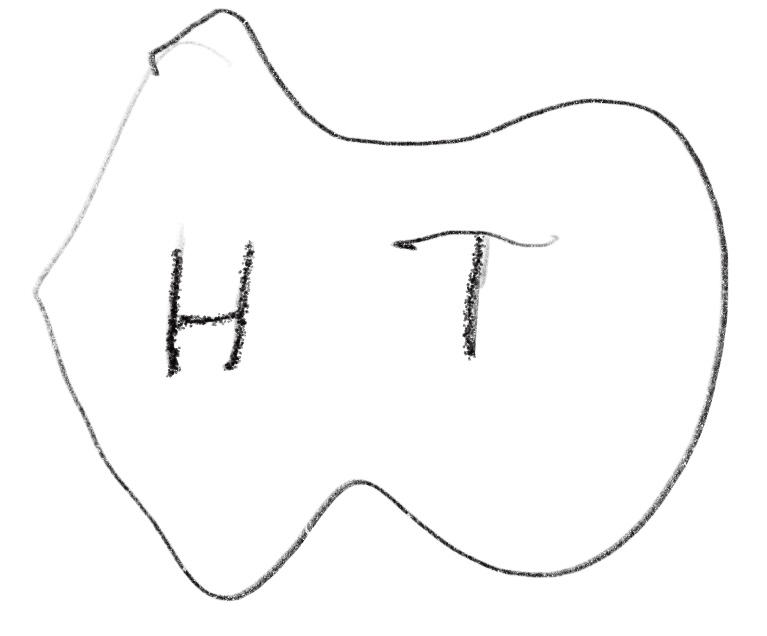
\includegraphics[width=5cm, height=4cm]{images/L01/IMG_1_1455.jpeg}
\caption{Missing}
\end{figure}

\begin{itemize}
    \item Sample space is a set
    \item Elements are the possible outcomes of the experiment
    \item Mutually exclusive
    \item Collectively exhaustive
\end{itemize}

\subsection{Example: 2 rolls of 4-sided die (tetrahedral die)}

% \reversemarginpar
\marginpar{(15:19)}
The experiment is both rolls (not 2 experiments)
% {(15:19)}

% 
\begin{figure}[ht]
\centering

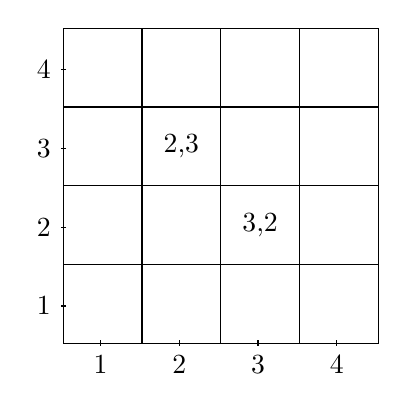
\begin{tikzpicture}
% \begin{axis}[
%     title={Unit Square},
%    height=8cm,width=8cm, 
%     xlabel={First Die},
%     x\ylabel={Second Die},
% ]
\draw (0,0) rectangle (4,4);
\draw (0,0) grid (4,4);
\foreach \x in {1,2,3,4}
   \draw[xshift=-15pt] (\x cm,1pt) -- (\x cm,-1pt) node[anchor=north] {$\x$};
\foreach \y in {1,2,3,4}
    \draw[yshift=-15pt] (1pt,\y cm) -- (-1pt,\y cm) node[anchor=east] {$\y$};

\draw (1.5,2.5) node{2,3};
\draw (2.5,1.5) node{3,2};
% \end{axis}
\end{tikzpicture}
\caption{2 4-Sided Die Roll Sample Space}
\end{figure}


Reserving the word "outcome" for the outcome of the overall experiment.

\subsection{Sequential Description}

\begin{figure}[ht]
\centering
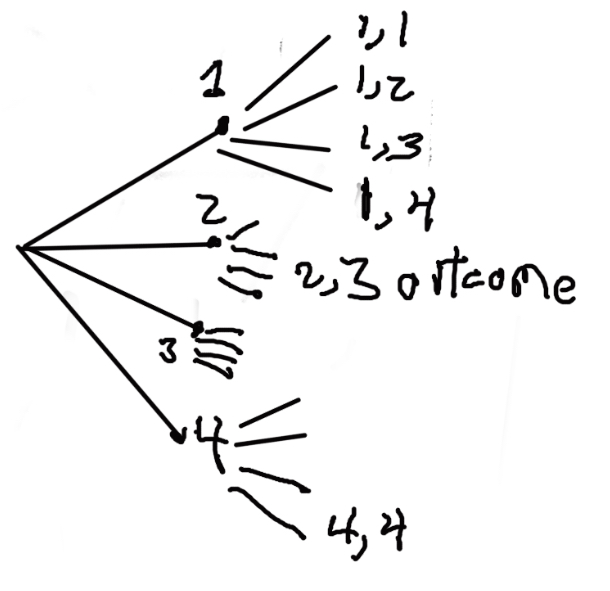
\includegraphics[width=5cm, height=4cm]{images/L01/sequential_desc.jpeg}
\caption{Sequential Description}
\end{figure}

\subsection{Sample Space: Continuous Example: Darts}

$\Omega = \{(x,y) | \quad 0 \le x, \quad y \le 1 \}$

\begin{figure}[ht]
\centering
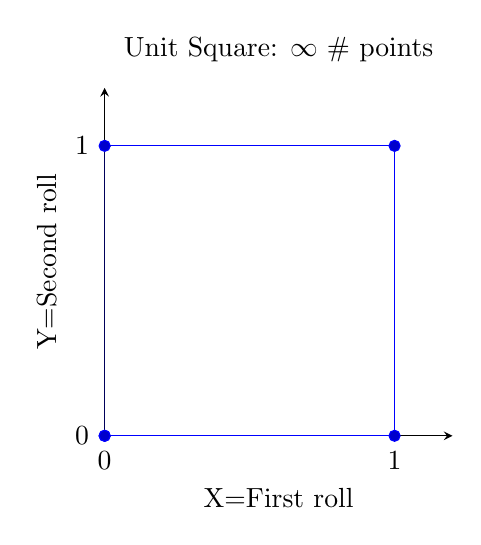
\begin{tikzpicture}
\begin{axis}[
    title={Unit Square: $\infty$ \# points},
   height=6cm,width=6cm, 
    axis lines = left,
    xmin=0, xmax=1.2,
    ymin=0, ymax=1.2,
    xlabel = \(x\),
    ylabel = {\(y\)},   
    xtick={0,1},
    ytick={0,1},
    xlabel={X=First roll},
    ylabel={Y=Second roll}
]
\addplot coordinates {
    (0,0)
    (0,1)
    (1,1)
    (1,0)
  (0,0)
     
};
\end{axis}
\end{tikzpicture}
\caption{Unit Square}
\end{figure}
We assign probabilities to the outcomes (not exactly).  Any individual point is zero.
\\
When we talk about the \textit{subsets} of sample space, we call them \textbf{events}.

\begin{figure}[ht]
\centering
    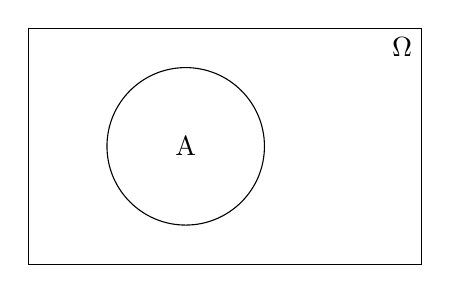
\begin{tikzpicture}
\draw (0,0) rectangle (5,3) node[anchor=north east] {$\Omega$};
\draw (2,1.5) circle (1cm) node {A};
\end{tikzpicture}
\caption{$\Omega$} \label{fig:M1}
\end{figure}


\subsection{Probability Axioms}

\begin{enumerate}
    \item Nonnegativity: \colorbox{yellow}{$P(A) > 0$}
    \item Normalization: $P(\Omega)=1$
    \item Additivity: If $A \cap B = \varnothing$, then $P(A \cup B)=P(A) + P(B)$
\end{enumerate}

\begin{figure}[!ht]
\centering
\begin{tikzpicture}
\draw (0,0) rectangle (7,4);
\draw (2,2) circle (1cm) node {A};
\draw (5,2) circle (1cm) node {B};
\end{tikzpicture}
\caption{A,B} \label{fig:M2}
\end{figure}

\begin{align*}
1 = P(\Omega) = P(A \cup A^c) \qquad \text{(by 2)}\\
= P(A) + P(A^c)  \qquad \text{(by 3)}\\
P(A) = 1 - P(A^c) \le 1  \qquad \text{(by 1)}\\
\end{align*}

Probabilities are always $\le 1$

\subsection{3 Events Union}

MISSING

\begin{figure}[!ht]
\centering
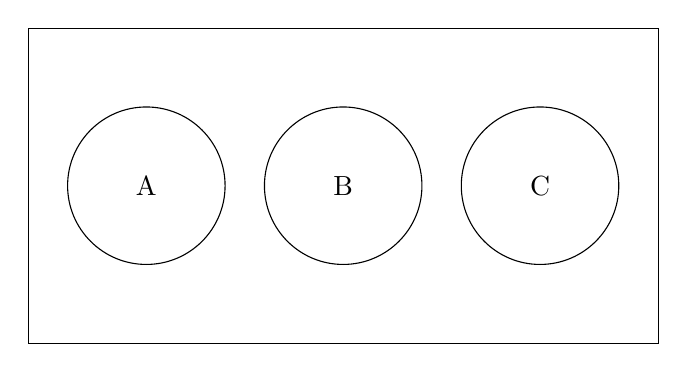
\begin{tikzpicture}
\draw (0,0) rectangle (8,4);
\draw (1.5,2) circle (1cm) node {A};
\draw (4,2) circle (1cm) node {B};
\draw (6.5,2) circle (1cm) node {C};
\end{tikzpicture}
\caption{A,B,C} \label{fig:M3}
\end{figure}

If $A_1,\ldots, A_n$ are disjoint then $P(A_1 \cup \cdots \cup A_n) = P(A_1) + \cdots + P(A_n)$

\begin{itemize}
    \item Axiom 3 has some issues \marginpar{(36:00)}
    \item Weird subsets.  Will ignore in this class.
\end{itemize}

\subsection{Discrete Uniform Law}

Model obeys this law if all outcomes are equally likely. (e.g. fair coins, fair dice, well-shuffled decks)

\subsection{Continuous Uniform Law}

\begin{figure}[!ht]
\centering
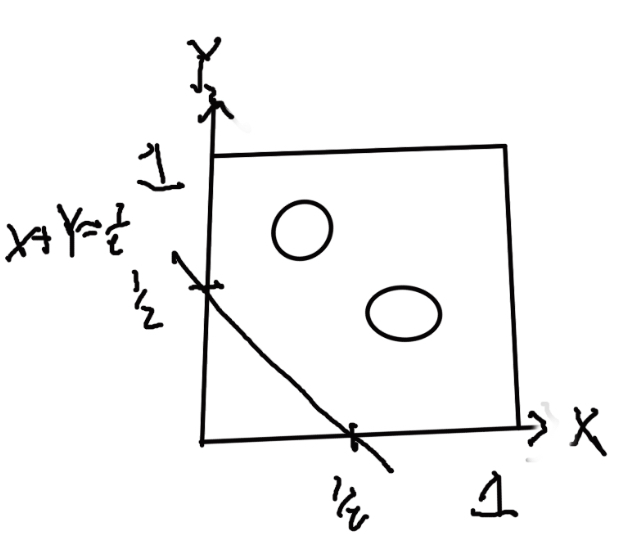
\includegraphics[width=5cm, height=4cm]{images/L01/cont_unif_law.jpeg}
\caption{x+y=1/2}
\end{figure}

\subsubsection{Uniform Law: Probability = Area}

\begin{align*}
P(X+Y \le \frac{1}{2}=? = \frac{1}{2} \frac{1}{2}\frac{1}{2} = \frac{1}{8}\frac{1}{2}b\cdot h\\
P((X,Y) = 0.5.0.3))= ? = 0 = \text{No area}
\end{align*}





\subsection{Example: Probability Law}

Countably infinite sample space.

equal areas = equal probabilities

\subsection{Countable Additivity Axiom}

If $A_1,\ldots, A_n$ are disjoint events, then can be arranged in order:

$$
P(A_1 \cup A_2 \cup \cdots) = P(A_1) + P(A_2) + \cdots
$$
Sequence of disjoint sets.
